% Analysis section
This section will outline colour construction, the clustering process, and the selection of the optimal clustering for each colour combination.
Each colour combination was clustered using the same process, and in two and three dimensions.

\subsection{Colour Selection}

An aim of this work was to help astronomers determine which filters are best at identifying different types of objects.
Since the average survey consists of four filters, different combinations of four filters were used to construct colours for clustering. 
Due to the large number of filters available in the ERS data, the combinations had to be narrowed down to a reasonable set.
Two types of colour combinations were created: combinations of all broad band filters, and combinations with one narrow band and three broad bands.
Additionally, two and three dimensions were considered for clustering, in order to maximize the use of the data in an average survey.

\subsubsection{Broad Band Combinations}

\textbf{PB: Should we explain what kind of objects we hope to find in these combos?}

The first type of combination was comprised of the broad band filters: F336W (U), F438W(B), F555W(V), and F814W(I).
The F225W (UVW) filter was not included in this set as it is not a standard filter most surveys.
Additionally, the $U - I$ colour was not used in the analysis because it was determined that this colour was not physically meaningful.
This is because it is unlikely that an object would emit a detectable reading in both these bands due to their distance from one another in wavelength.
Using the four filters, the broad band colour combinations created can be found in Table~\ref{tab:BBcolours}.
These combinations were created in order to remove any obvious correlation between the colours that could occur by the inclusion of the same band in both colours.

\begin{table*}
\centering
\caption{Broad band colour combinations and the number of objects detected in each colour, and in each combination, with uncertainties less than $0.2$.}
\label{tab:BBcolours}
\begin{tabular}{lllllll}
\hline\hline
Colour 1 & Objects & Mean Uncertainty & Colour 2 & Objects & Mean Uncertainty & Combined Objects \\
\hline
$U - B$ &  33523 & 0.1606 mag & $V - I$ &  57935 & 0.1334 mag & 28931\\
$U - V$ &  33692 & 0.1429 mag & $B - I$ &  41413 & 0.1590 mag & 28931\\
$B - V$ &  48660 & 0.1456 mag & $ - $ & $ - $ & $ - $ & $ - $ \\
\hline
\end{tabular}
\end{table*}

\subsubsection{Narrow Band Combinations}

\textbf{PB: Should we explain more about why we choose to do Broad - Narrow? And what objects we hope to find in these combos?}

The second set of combinations included the narrow band filters: F373N ($O_{2}$), F487N ($H\beta$), F502N ($O_{3}$), F657N ($H\alpha$), and F673N ($S_{2}$).
In addition, the broad band F225W (UVW) was included in this set to ensure its data was included in the analysis. 
Colours were created with the narrow bands by pairing them with the broad bands that covered them in wavelength space.
These colours were created in order to reduce the number of possible combinations that could be used for analysis.
The second colour in each combination was created from two broad bands that did not overlap the first colour in wavelength space.
Table~\ref{tab:NBcolourcombos} lists the narrow band colour combinations used for analysis.
The number of objects in the narrow band combination, with the exception of the $H\alpha$ band, is significantly lower than the broad band combinations.
These combinations were useful for analysis as their distributions were not as dense as the broad bands, and the clustering algorithms were able to detect interesting structure within them.
Making colours out of a combination of broad and narrow bands ensure that the objects clustered in these bands are physically meaningful, as it is likely that the object would emit in the broad band that contains the narrow band. \textbf{Not sure if that is a reason why we chose to construct them that way}.

\begin{table*}
\centering
\caption{Narrow band colour combinations and the number of objects detected in each colour, and in each combination, with uncertainties less than $0.2$.}
\label{tab:BBcolours}
\begin{tabular}{lllllll}
\hline\hline
$Narrow - Broad$ & Objects & Mean Uncertainty & $Broad - Broad$ & Objects & Mean Uncertainty & Combined Objects \\
\hline
$UVW - U$ &  14977 & 0.1539 mag & $B - V$ &  48660 & 0.1456 mag & 14943 \\
$ - $ & $ - $ & $ - $ & $B - I$ &  41413 & 0.1590 mag & 14095 \\
$ - $ & $ - $ & $ - $ & $V - I$ &  57935 & 0.1334 mag & 14098 \\
\hline
$U - O_{2}$ & 8675 & 0.1504 mag & $B - V$ &  48660 & 0.1456 mag & 8657 \\
$ - $ & $ - $ & $ - $ & $B - I$ &  41413 & 0.1590 mag & 8558 \\
$ - $ & $ - $ & $ - $ & $V - I$ &  57935 & 0.1334 mag & 8559 \\
\hline
$B - H\beta$ & 13269 & 0.1493 mag & $V - I$ &  57935 & 0.1334 mag & 13147 \\
\hline
$O_{3} - V$ & 14644 & 0.1418 mag & $U - B$ &  33523 & 0.1606 mag & 13390 \\
\hline
$H\alpha - I$ & 59465 & 0.1495 mag & $U - B$ &  33523 & 0.1606 mag & 28920 \\
$ - $ & $ - $ & $ - $ & $U - V$ &  33692 & 0.1429 mag & 29060 \\
$ - $ & $ - $ & $ - $ & $B - V$ &  48660 & 0.1456 mag & 41317 \\
\hline
$S_{2} - I$ & 25185 & 0.1535 mag & $U - B$ &  33523 & 0.1606 mag & 14577 \\
$ - $ & $ - $ & $ - $ & $U - V$ &  33692 & 0.1429 mag & 14586 \\
$ - $ & $ - $ & $ - $ & $B - V$ &  48660 & 0.1456 mag & 18882 \\
\hline
\end{tabular}
\end{table*}

\subsubsection{Number of Dimensions}
Due to the high number of bands available in the ERS data, the number of dimensions available to cluster was very high.
Limiting the number of band combinations through the system outlined above helped reduce the number of dimensions.
However, in addition to the two dimensional combinations, clustering in three dimensions was investigated.
Three dimensional colour combinations were created based on the combinations listed in Table~\ref{tab:BBcolours} and Table~\ref{tab:NBcolourcombos}.
In the broad band combinations, three dimensional colour spaces were created by making colours with a common band, either B or V.
These bands were selected in order to avoid creating the $U - I$ colour.
\textbf{PB: Not sure if this next sentance explains why we chose to use a common band clearly. Just trying to say that the colours could be subtracted to transform back into the two dimensional space.}
A common band was used in all colours in order to create a three dimensional space that of colours that could be transformed back into the original two dimensional space. 

In the narrow band combinations, the three dimensional colour spaces were created by making colours with the narrow band common between them.
Similar to the broad band spaces, these combinations could be transformed into the original two dimensional space, and act as an extension of the two dimensional distribution.

Clustering in three dimensions increased the complexity of the distribution, creating more information for the clustering algorithms to use.
However, limiting the dimensionality of the problem to three allowed the analysis to stay within the constraints of a common survey.
A space of up to 45 dimensions could have been created, but that space would not be reasonable for the analysis of a common survey.

\subsection{Clustering Process}
Clustering was performed using all methods for each colour combination. 
The following process allowed the investigation of the effect of all paramters on each clustering technique, leading to the selection of an optimal clustering.

\subsubsection{Meanshift}
Mean-Shift clustering was performed first by estimating the bandwidth paramter with the $estimate-bandwidth$ function in $scikit-learn$. \textbf{How do we cite this package?}
This function estimates the bandwidth parameter based on the distances between points in the dataset, and determines if the distribution has high or low variance.
Following the initial clustering, a the bandwidth was varried and the clustering was performed again with bandwidth values on intervals of $\pm 0.1$ from the estimated bandwidth value.
Varying the bandwidth revealed how sensitive a combination was to the parameter.
If a combination was very sensitive to bandwidth, then the number of clusters that meanshift would predict would vary greatly over a small range of bandwidth values.
This type of combination usually resulted in poor segmentation, as the algorithm would not converge on a number of clusters. 
However, sensitivity could also be the result of the starting bandwidth estimate.
If the original estimate was in an unstable bandwidth interval, then the hierarchy would reflect that, and the testing of multiple bandwidth values could result in convergence.

\subsubsection{Affinity Propagation}
Affinity Propagation clustering was performed after Meanshift. 
The first clustering was run using the preference estimations outlined in Section 3. \textbf{how to referene section}.
The preferences were set to the median and the minimum value of the similarities, and the damping factor was kept at the default value of $0.5$.
This resulted in a segmentation with over 100 clusters in multiple colour combinations.
The preferences were then set to 10\% of the number of objects in the data set, and the damping factor was set at $0.95$.
With these parameters, the clusterings varried significantly over differnet colours. 
The clusterings were repeated to try and reveal a trend in the parameters, but the algorithm was too sensitive for this size of dataset.
Following the initial tests of Affinity Propagation, it was determined that this clustering method was not effective.
Due to the number of computations required for the calculation of the messages passed between points on each iteration, the algorithm was very sensitive to the input parameters, and did not produce meaningful clusterings.
The algorithm is effective for small and medium sized datasets, and was able to create some reasonable clusters when the uncertainty limit was set at $0.1 mag$, which reduced the number of objects significantly. 
After multiple clusterings, a systematic way of determine the correct number of clusters could not be determined, and the algorithm was not used further.

\subsubsection{K-Means}
K-Means clustering was performed last.
The first clustering was performed using the number of clusters determined from the initial clusterings by Meanshift.
Next, K-Means was performed with $K = \pm 4$ from the original clustering.
This method of clustering was similar to the Meanshift approach, as it revealed how the dataset reacted to different values of $K$.
K-Means was the most efficient algorithm of the three, as it produced clusterings quickly, and always produced clusters of reasonable size.

\subsection{Selecting the Optimal Clustering}
Determining the optimal clustering was the most difficult task of the analysis.
Selecting the optimal clustering can often seem arbitrary, as no ``right" answer is obvious.
In order to determine the optimal clustering, a variety of metrics and statistics were calculated to evaluate each cluster.
Additionally, the relationships between a variety of clustering parameters were investigated to try and determine where they indicated the optimal clustering.
Since the performance of the algorithms was directly related to the parameters used as input, those relationships were critical for selecting the clustering.
The objects in each cluster were then found in the white-light image of M83, to determine if there was a relationship between the objects assigned to the same cluster and their spatial position.
Finally, colour models were created and imposed on the cluster distribution to determine if the segmentation agreed with a model. \textbf{Need more on why the models were used}.

\subsubsection{Silhouette Score}
The silhouette score is a metric used to describe the compactness of a cluster in a given clustering and is calculated as an average of all samples in a clustering.  
The silhouette score is given by:

\begin{equation}
\label{eq:ss}
Silhouette Score = \frac{b - a}{\textit{max}\big(a, b\big)}
\end{equation}

where $a$ is the mean intra-cluster distance, and $b$ is the distance between a point and the nearest cluster that point is not a member of.
The score was used in two ways.
First, the average score was calculated for a given clustering.
This calculated the average score across all data in the sample.
Next, the average score for each cluster was computed.
The average cluster score evaluates the strength of a given cluster within a clustering.
This metric allowed each cluster to be evaluated individually, and revealed which clusters were responsible for the average score of the clustering.
Additionally, the average score allowed seemingly arbitrary clusters to be evaluated.
If the segmentation did not seem meaningful, the average score would reveal if the cluster was isolated and compact.
This revealed the significance of clusters that could have been viewed as noise or outliers. \textbf{This section needs more explaination}.

\textbf{Struggling to explain why that is how the score works}. 
Ideally, the silhouette score for the entire clustering should peak near the center of the distribution indicating the optimal clustering. 
High scores where the number of clusters is low often do not reflect the structure of the distribution, while high numbers of clusters are often imposed on the data as a result of the specified parameters.
This is often not the case, as seen in Figure~\ref{fig:sscore}, which shows the distribution of the silhouette score against the number of clusters.
For the K-Means clusterings, the score does not peak in the center of the distribution.
Instead of selecting the clustering with the highest score, the optimal clustering is found where the relation begins to elbow; between 4 and 5 clusters.
This clustering is selected because any increase in $K$ after this point does not affect the score, and does strengthen or weaken the clustering.
This means that the algorithm has found the balance between the natural clusters in the distribution and artificially segmenting the data.

\begin{figure}[H]
\centering
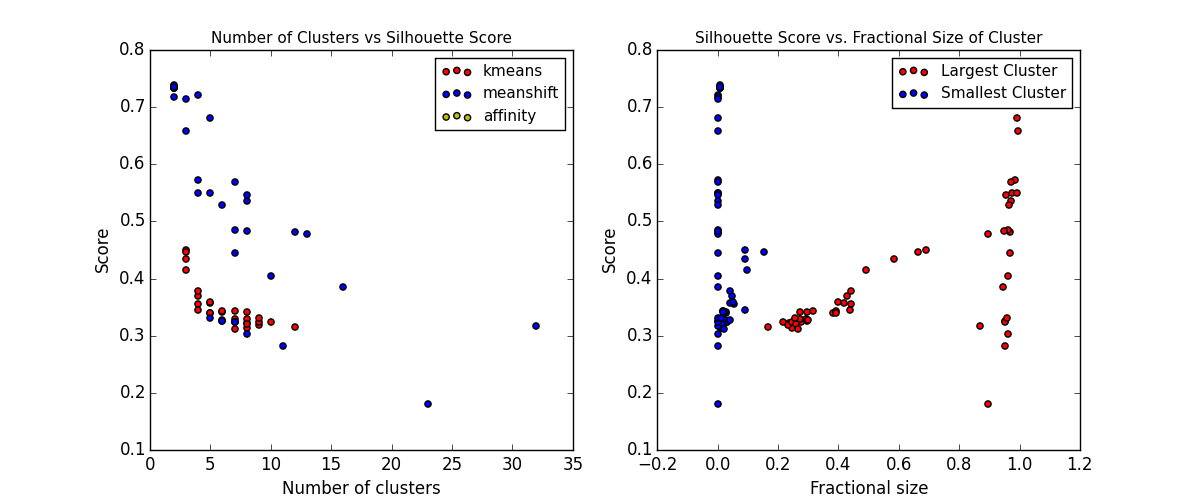
\includegraphics[width=\linewidth]{figs/methods/silhouette_score_relation}
\caption{Distribution of the silhouette score as a result of the number of clusters imposed for the $UVW - U$ and $V - I$ colours. The \textit{blue} points are the scores of Meanshift clustering, \textit{red} points are scores of K-Means.}
\label{fig:sscore}
\end{figure}

The distribution of score as a result of the Meanshift algorithm does not follow the same pattern.
The silhouette score was not as successful at describing the strength of Meanshift clusterings as Meanshift often created one large cluster and several smaller ones, which is not considered strong by the score.
In order to determine the optimal Meanshift clustering, other relationships were investigated.

\subsubsection{Cluster Statistics}
Various statistics were calculated to help describe the similarity between the objects in a given cluster.
The standard deviation and average colour was calculated for each colour, and each cluster within a clustering. 
These metrics helped describe the distribution of the objects in the colour-colour space within a cluster. 
Clusters that had large standard deviations were viewed as too dissimilar to be a meaningful cluster, and clusters whose averages varried significantly from the cluster centers were disgarded.

\textbf{I'm not sure that this paragraph describes why we calculated the fractional size}.
The fractional size of each cluster was also calculated and described the distribution of objects between clusters.
If a clustering segmented the objects into a large cluster followed by several smaller ones, the clustering was investigated further, as this segmentation could mean one of two things. 
This type of clustering could be a result of the identification of interesting objects, in which case the clustering algorithm was able to identify the objects and place them in the same cluster.
However, this type of clustering could also be a result of the underlying distribution of the data, as the clustering techniques are largely drawn to areas of high density.
If this is the case, the clustering only created the smaller clusters as a result of the parameters imposed on the clustering.

\subsubsection{Parameter Relationships}
In addition to metrics, the relationships between various parameters were investigated to determine how the each clustering method behaved.

Each K-Means clustering was checked by plotting the sum-of-squares value for each value of $K$.
Figure~\ref{fig:inertia} shows the inertia distribution for the $H\beta - B$ vs. $V - I$ colour.
As $K$ increases, the inertia value decreases as the inertia value represent the total distance between the total distance between the points of each cluster.
The value decreases with $K$ as the total distance in each cluster decreases as more clusters are introduced.
This distribution was used to check the clustering and ensure that the clusterings were successful.

\begin{figure}[H]
\centering
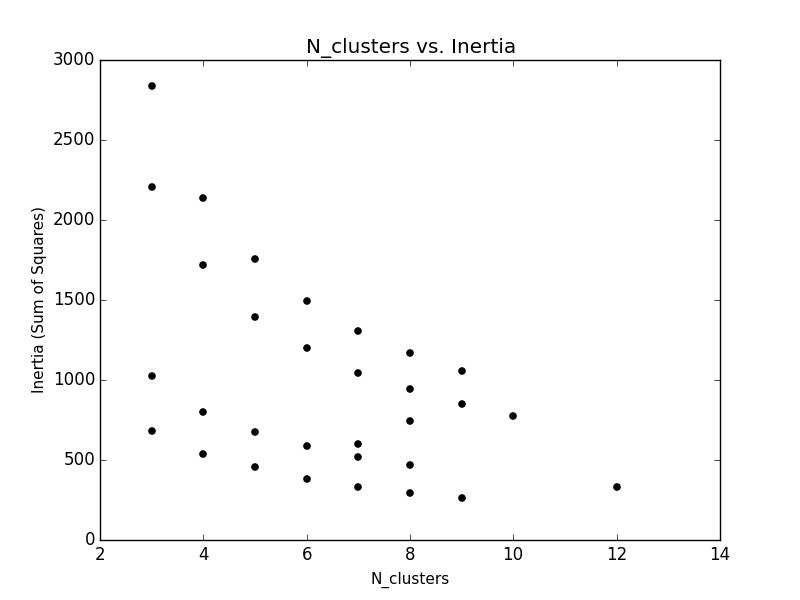
\includegraphics[width=\linewidth]{figs/methods/inertia_plot}
\caption{Distribution of the inertia as a result of the number of clusters for the $H\beta - B$ and $V - I$ combination.}
\label{fig:inertia}
\end{figure}

The behavior of the bandwidth parameter was investigated for each Meanshift clustering.
Figure~\ref{fig:bad_ms} shows the relation between the score and number of clusters for the three dimensional $U - O_{2}$ and $B - I$ combination.
The blue dots represent the Meanshift clusterings.

\begin{figure}[H]
\centering
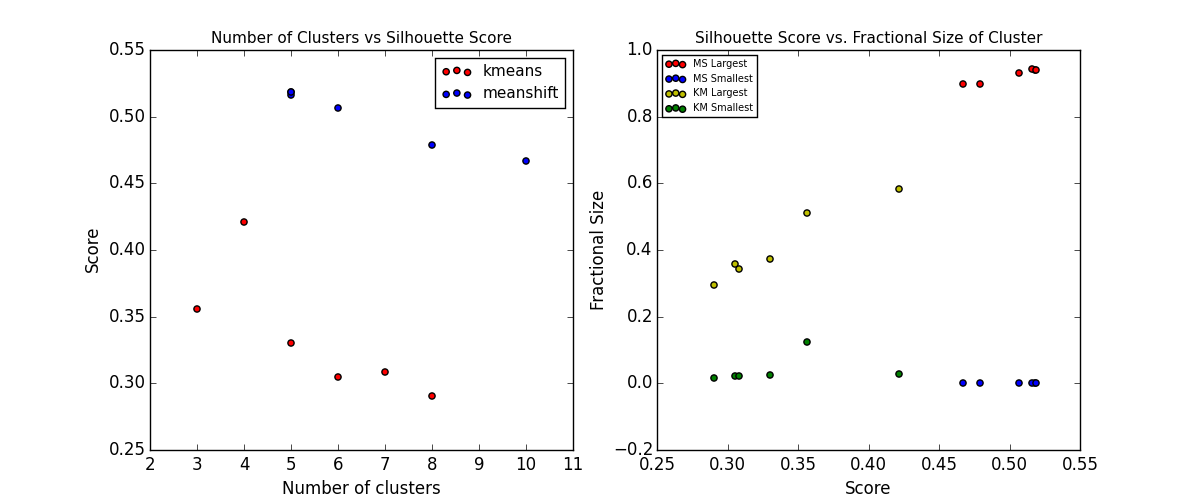
\includegraphics[width=\linewidth]{figs/methods/silhouette_score_bad_ms}
\caption{Distribution of the silhouette score as a result of the number of clusters imposed for the three dimensional $U - O_{2}$ and $B - I$ combination. The \textit{blue} points are the scores of Meanshift clustering, \textit{red} points are scores of K-Means.}
\label{fig:bad_ms}
\end{figure}

It is clear that an optimal clustering cannot be determined from this relation, as the score decreases linearly with the number of clusters Meanshift predicts.
The Mean-Shift scores do not follow a similar distribution as K-Means, as the accuracy of Meanshift is related to the bandwidth parameter, seen in Figure~\ref{fig:bwscore}.
The optimal Mean-Shift clustering was chosen by finding the bandwidth where the relation between the bandwidth and number of clusters reached an elbow, or where the relation between bandwidth and silhouette score elbowed.
In both panels of Figure~\ref{fig:bwscore} that the bandwidth parameter predicts five clusters.
Both distributions elbow at the same bandwidth interval, maximizing the score and predicting the same number of clusters for bandwidth valeus following the elbow.
The bandwidth parameter was the primary indicator of the optimal Meanshift clustering.
If a trend could not be found with the bandwidth parameter, then the silhouette score and number of clusters was investigated.

\begin{figure}[H]
\centering
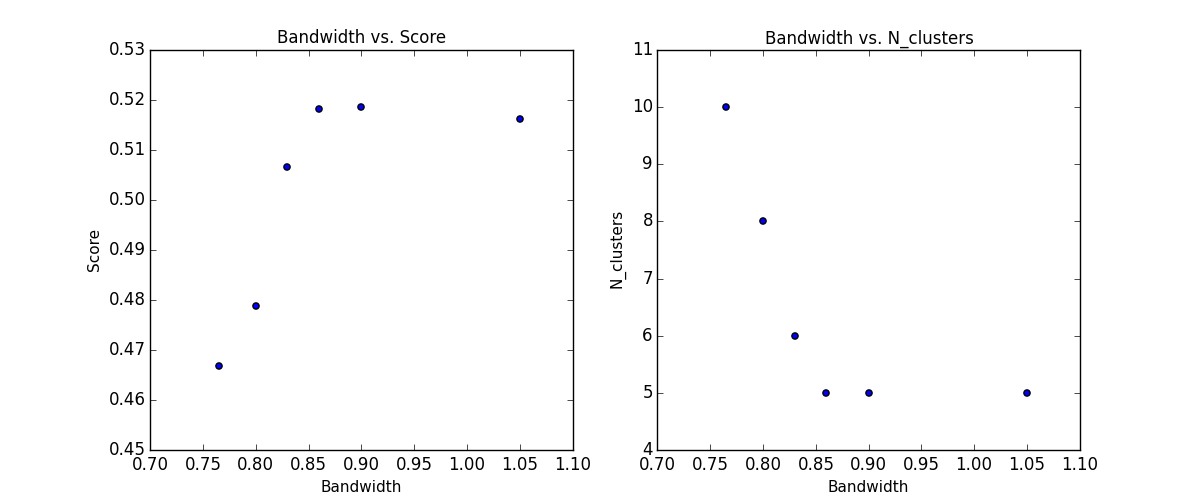
\includegraphics[width=\linewidth]{figs/methods/meanshift_parameters}
\caption{Distribution of the silhouette score as a function of bandwidth, and the distribution of the number of clusters as a function of bandwidth.}
\label{fig:bwscore}
\end{figure}